\chapter{Cryptocurrency Exchanges}
\label{ch:exchanges}

In this chapter, we describe different exchange types and characteristics in more detail and provide a selection of several exchanges. We will outline what to look out for when you look for an exchange and identify the general steps involved when you sign up.

\medskip

\section{What are cryptocurrency exchanges}
A cryptocurrency exchange is a marketplace where you can buy, sell or exchange cryptocurrencies for other digital cryptocurrencies and traditional [digital] currencies like US dollars or Euros. If you want to trade professionally and have access to fancy trading tools, you will likely need to use an exchange that requires you to verify your ID and open an account (known as the \emph{Know Your Customer} protocol). If you want to make the occasional, straightforward trade, there are also platforms that you can use that do not require an account. There are four different types of cryptocurrency exchanges that you can use to trade and buy coins. Understanding the differences between the exchanges is the essential first step to choosing the best cryptocurrency exchange for you. But before this, an important aspect of exchanges and trading, in general, will be discussed.

\begin{enumerate}[label=(\alph*)]
  \setlength\itemsep{0em}
    \item Broker Exchanges (\cref{subsec:broker_exchange})
        \begin{itemize}
            \item Mostly centralized and primarily used to buy crypto with fiat currency. %(\cref{subsubsec:CEX}).
        \end{itemize}
    \item Trading Exchanges (\cref{subsec:trading_exchange})
        \begin{itemize}
            \item Can be both centralized or decentralized and is primarily used to trade crypto to crypto.
            \item Nowadays, some trading exchanges enable you to buy crypto directly using traditional payment methods such as credit cards and PayPal. %(\cref{subsubsec:DEX}).       
            \end{itemize}
\end{enumerate}

\section{Converting FIAT into cryptocurrency}
 Once registered on an exchange that allows for currency deposits, you can start to engage the market. You now have a host of different options available, depending on the available trading pairs for the currency you deposited. Depending on your country and the currency you're using - you will most likely end up using a broker exchange that operates either internationally and offers multiple currency trading pairs or a local one that also deals in your currency. Trading pairs that you will find almost everywhere would be Bitcoin and Ethereum (USD/BTC, USD/ETH, EUR/BTC, and EUR/ETH). Have a look at the trading pairs available for your currency at your broker exchange. You can deposit money on your exchange account in multiple ways (depending on your provider). You might be able to use bank deposits (SEPA), credit cards or perhaps even services like PayPal.\medskip

As mentioned before, not all types of exchanges accept fiat currency deposits (broker exchanges only); some exchanges only allow you to deposit cryptocurrencies to exchange other alternative coins (trading exchanges). Today, Bitcoin is still one of the most popular cryptocurrencies, and all exchanges offer Bitcoin. Therefore, you can consider it as one of the best gateways for purchasing other coins. In other words, if you want to buy any other cryptocurrencies, you must look at the trading pairs available and do the following:

\begin{enumerate}
    \item Open a (domestic) cryptocurrency broker exchange account (in your country) and verify your account via the "Know Your Customer" (KYC) protocol if required. Please refer to \cref{subsec:broker_exchange} for more information on broker exchanges.
    \item Deposit funds from your bank account to your broker crypto exchange account so you can buy Bitcoin, Ethereum or another coin that has high liquidity and offers multiple trading pairs.
    \item Open a trading exchange account that offers a variety of other cryptocurrencies. Usually, these exchanges do not accept fiat deposits and only allow crypto to crypto trading, withdrawals and deposits. Please refer to \cref{subsec:trading_exchange} for more information on trading exchanges.
    \item After verifying your account, transfer the cryptocurrency that you've bought from your broker exchange to your new trading exchange, and you can start trading. If you don't know how to transfer your freshly purchased coins out of your accounts, please refer to \cref{ch:wallets} where we discuss wallets and transactions.
\end{enumerate}

\newpage

\section{Market liquidity}
Cryptocurrency exchanges, like all exchanges, have to deal with (il)liquidity. The cryptocurrency market itself is highly volatile and contains many relatively liquid (high market capitalization and trade volume) but also plenty of illiquid (hard to sell quickly due to a lack of ready and willing buyers) cryptocurrencies. 

Liquidity describes the extent to which an asset or security can be quickly bought or sold in the market without affecting the asset price. Liquid assets are relatively easy to buy and sell, and the majority of people and businesses accept liquid assets as a means of payment.

    \bigskip  
    \begin{cryptobox}{\textbf{LIQUID CASH}}
        \textit{The prime example of a liquid asset is cash. Everybody accepts cash, and you can use cash almost anywhere in the world, although when traveling internationally you might have to exchange your cash currency for another currency based on your destination. The cash markets are so liquid that there is little to no volatility and exchange rates are generally very stable.}
    \end{cryptobox}
    \medskip

Keep in mind that this principle of liquidity and the relation to asset price applies to any market and asset. Some more examples of fairly liquid assets include stocks, bonds, and listed commodities, including precious metals such as gold and silver. These liquid assets can be sold almost instantaneously during regular market hours at fair value.

When choosing an exchange for buying and selling cryptocurrencies - take into account the trade volume of your exchange and consider your entry and exit strategy. Among others, look at the available options offered by various exchanges, trading pairs, and possibilities to use fiat currency. Bitcoin (BTC) dominates the market up to this day, but there are plenty of other smaller projects competing for a position in the top 100. 

There are thousands of cryptocurrency projects, but simultaneously, there are numerous exchanges where all of these assets are sold, which is part of the problem. Essentially, the exchanges are competing with each other for liquidity in a relatively small market with relatively low market capitalization. 

\section{Exchange types}
\label{sec:exchangetypes}

There are plenty of exchanges available which operate in your geographic location. If you're interested in purchasing a particular project, coin or token, you can use CoinMarketCap and CoinGecko as shown in \cref{tab:exchangeoverview}.
Here you navigate to the specific asset or exchange, and you'll have access to a world of information, which you're able to filter. This overview is precious if you're looking for popular exchanges, exchanges with high volume, exchanges that list many coins or tokens or exchanges that have been around for years. In short, we believe such aggregated sites are a perfect place to start exploring.


\begin{table}

\centering

\caption{Starting points to learn about exchanges}

\begin{tabular}{ll} 
\toprule

\textbf{Platform} & \textbf{URL}\\
\midrule

CoinMarketCap   & \href{https://coinmarketcap.com}{coinmarketcap.com}      \\
CoinGecko       & \href{https://www.coingecko.com/en}{coingecko.com}    \\
CoinCheckup & \href{https://coincheckup.com}{coincheckup.com}    \\
CryptoCompare   & \href{https://www.cryptocompare.com}{cryptocompare.com}  \\
CoinPaprika      & \href{https://coinpaprika.com}{coinpaprika.com}         \\


\bottomrule
\end{tabular}
\label{tab:exchangeoverview}
\end{table}



\section{Centralized versus decentralized exchanges}
\label{sec:centralizedvsdecentralized}

In the field of cryptocurrencies, exchanges are mainly divided into decentralized exchanges and centralized exchanges. Leading exchanges such as Binance, Coinbase, and Huobi are all of centralized nature, which are challenged by problems of opaque trading rules, in-transparent fund storage, and security. Decentralized exchanges hope to capitalize on many of the security problems faced by centralized exchanges. However, we conclude that decentralized exchanges - although very safe - are not yet popular among the general public and need a higher level of user-friendliness, especially liquidity, to attract more users. \medskip


In terms of the development of decentralized exchanges, inevitable trade-offs still have to be made, as shown in \cref{tab:centralizedvsdecentralized}. However, this is progressing and expected to change in the (near) future. You will likely need to register at least one centralized broker exchange that allows you to enter the market by depositing fiat currency. After making your first deposit, you are ready for your first trade (purchase of digital assets) and send your newly acquired assets to a decentralized or centralized trading exchange as you deem fit.\medskip



\begin{table}[htb]

\centering

\caption{Centralized versus decentralized exchanges}
\begin{tabular}{lcl} 
\toprule
\textbf{Decentralized}         & & \textbf{Centralized}                 \\
\midrule
User controls funds       &$\longleftrightarrow$      & Exchange controls funds              \\
Anonymous            &$\longleftrightarrow$           & Not anonymous                        \\
No hacks and server down-time &$\longleftrightarrow$  & Hacks and server down-time possible  \\
Not (yet) user-friendly    &$\longleftrightarrow$     & Fairly user-friendly                 \\
Low trading volume (illiquidity) &$\longleftrightarrow$ & High volume (liquidity)              \\
Basic trading options and tools&$\longleftrightarrow$ & Advanced options and tools           \\
\bottomrule
\end{tabular}
\label{tab:centralizedvsdecentralized}
\end{table}



\subsubsection{Decentralized exchanges (DEX)}

A decentralized exchange or DEX is an exchange that allows you to trade cryptocurrency with other people utilizing the blockchain directly. Unlike a centralized exchange, you don't need a "middleman"; there is no central authority or main server required to make a transaction. In this sense, you could use it in the same way as a centralized exchange, although they usually have a lower trade volume (fewer buyers and sellers) and might be a little less user-friendly in terms of user interface and user experience (UI/UX). However, the landscape is changing rapidly as technology advances, and more and more DEXs emerge. 

\medskip

\begin{cryptobox}{\textbf{YOUR OWN CENTRAL BANK}}

When you are not in control of your private keys and instead have your funds stored in a hot wallet on a custodial exchange account (i.e. Coinbase), you don't truly own your cryptocurrencies and thus run additional and unnecessary risks. By converting fiat currency into cryptocurrencies, you can store your assets in such a way that only you can access them, you have full control at any time, without counterparty risk.

\tcblower
Remember; \textbf{not your keys - not your crypto.}

\end{cryptobox}

\medskip

\subsubsection{Centralized exchange (CEX)}
Centralized exchanges are the weakest link in the cryptocurrency community, and a chain is only as strong as its weakest link. Ironically, most existing digital currency exchanges built within the cryptocurrency ecosystem are centralized, making them vulnerable in ways our digital currencies are not.
A centralized exchange such as Coinbase, Kraken or Binance is run by a profit-oriented company that gets revenue from their platform's fee structures. Both the access and exit points into the current blockchain ecosystem require fees - all of which go to the centralized exchanges that facilitate these services. The counterparty risk and high fees are the main reasons why decentralized exchanges are needed. In all honesty, it is worth mentioning that many centralized exchanges can execute fiat currency to cryptocurrency transactions while DEXs, on the other hand, are usually only able to facilitate crypto to crypto transactions (for now). Signing up for an exchange can be cumbersome due primarily to Know Your Customer (KYC), Anti Money Laundering (AML) and other regulations when it comes to interfacing with traditional financial infrastructures. We will go back to this in our chapter about cryptocurrency wallets (\cref{ch:wallets}). 

\medskip

\section{Broker exchanges}
\label{subsec:broker_exchange}

A broker exchange allows you to buy crypto directly with your local currency. In other words, with a broker exchange, you can effectively convert your fiat currency for cryptocurrency or cash out your crypto and convert it back to fiat currency. A broker exchange is required for beginners and is your starting point if you don't have any cryptocurrency assets in the game which you can trade. 


\subsection*{Coinbase}
\href{https://www.coinbase.com/join/51954a2b26a1bcc484000015}{Coinbase} is, without a doubt, one of the most well-known exchanges in the world. Coinbase is one of the largest broker exchanges, very user-friendly but charges relatively high fees. At Coinbase, you can buy and sell the most well-known cryptocurrencies such as Bitcoin and Ethereum by simply registering, linking your bank account and making a deposit. You can make deposits in almost all fiat currencies, provided that Coinbase is operating in your country (check \href{https://support.coinbase.com/}{Coinbase Support}). Once your account is credited, you will receive a notification through email that you can now exchange your freshly deposited fiat currency for the cryptocurrency of your choice. Their website offers multiple web wallets in which you can store and hold your coins. From here, you can send and receive payments, deposit and withdraw (cash-out) to your bank account. 

    \bigskip
    \begin{topbox}{TIP}
    Sign up with \href{https://www.coinbase.com/join/51954a2b26a1bcc484000015}{Coinbase} using {\fontseries{extrabold}\selectfont cryptomanuals'} affiliate link and receive a bonus of \euro 8 worth of Bitcoin on top of your first deposit of \euro 100.
    \tcblower
    Learn more? Check \href{https://support.coinbase.com/}{Coinbase Support}.
    \end{topbox}
    
    \begin{borderbox}
        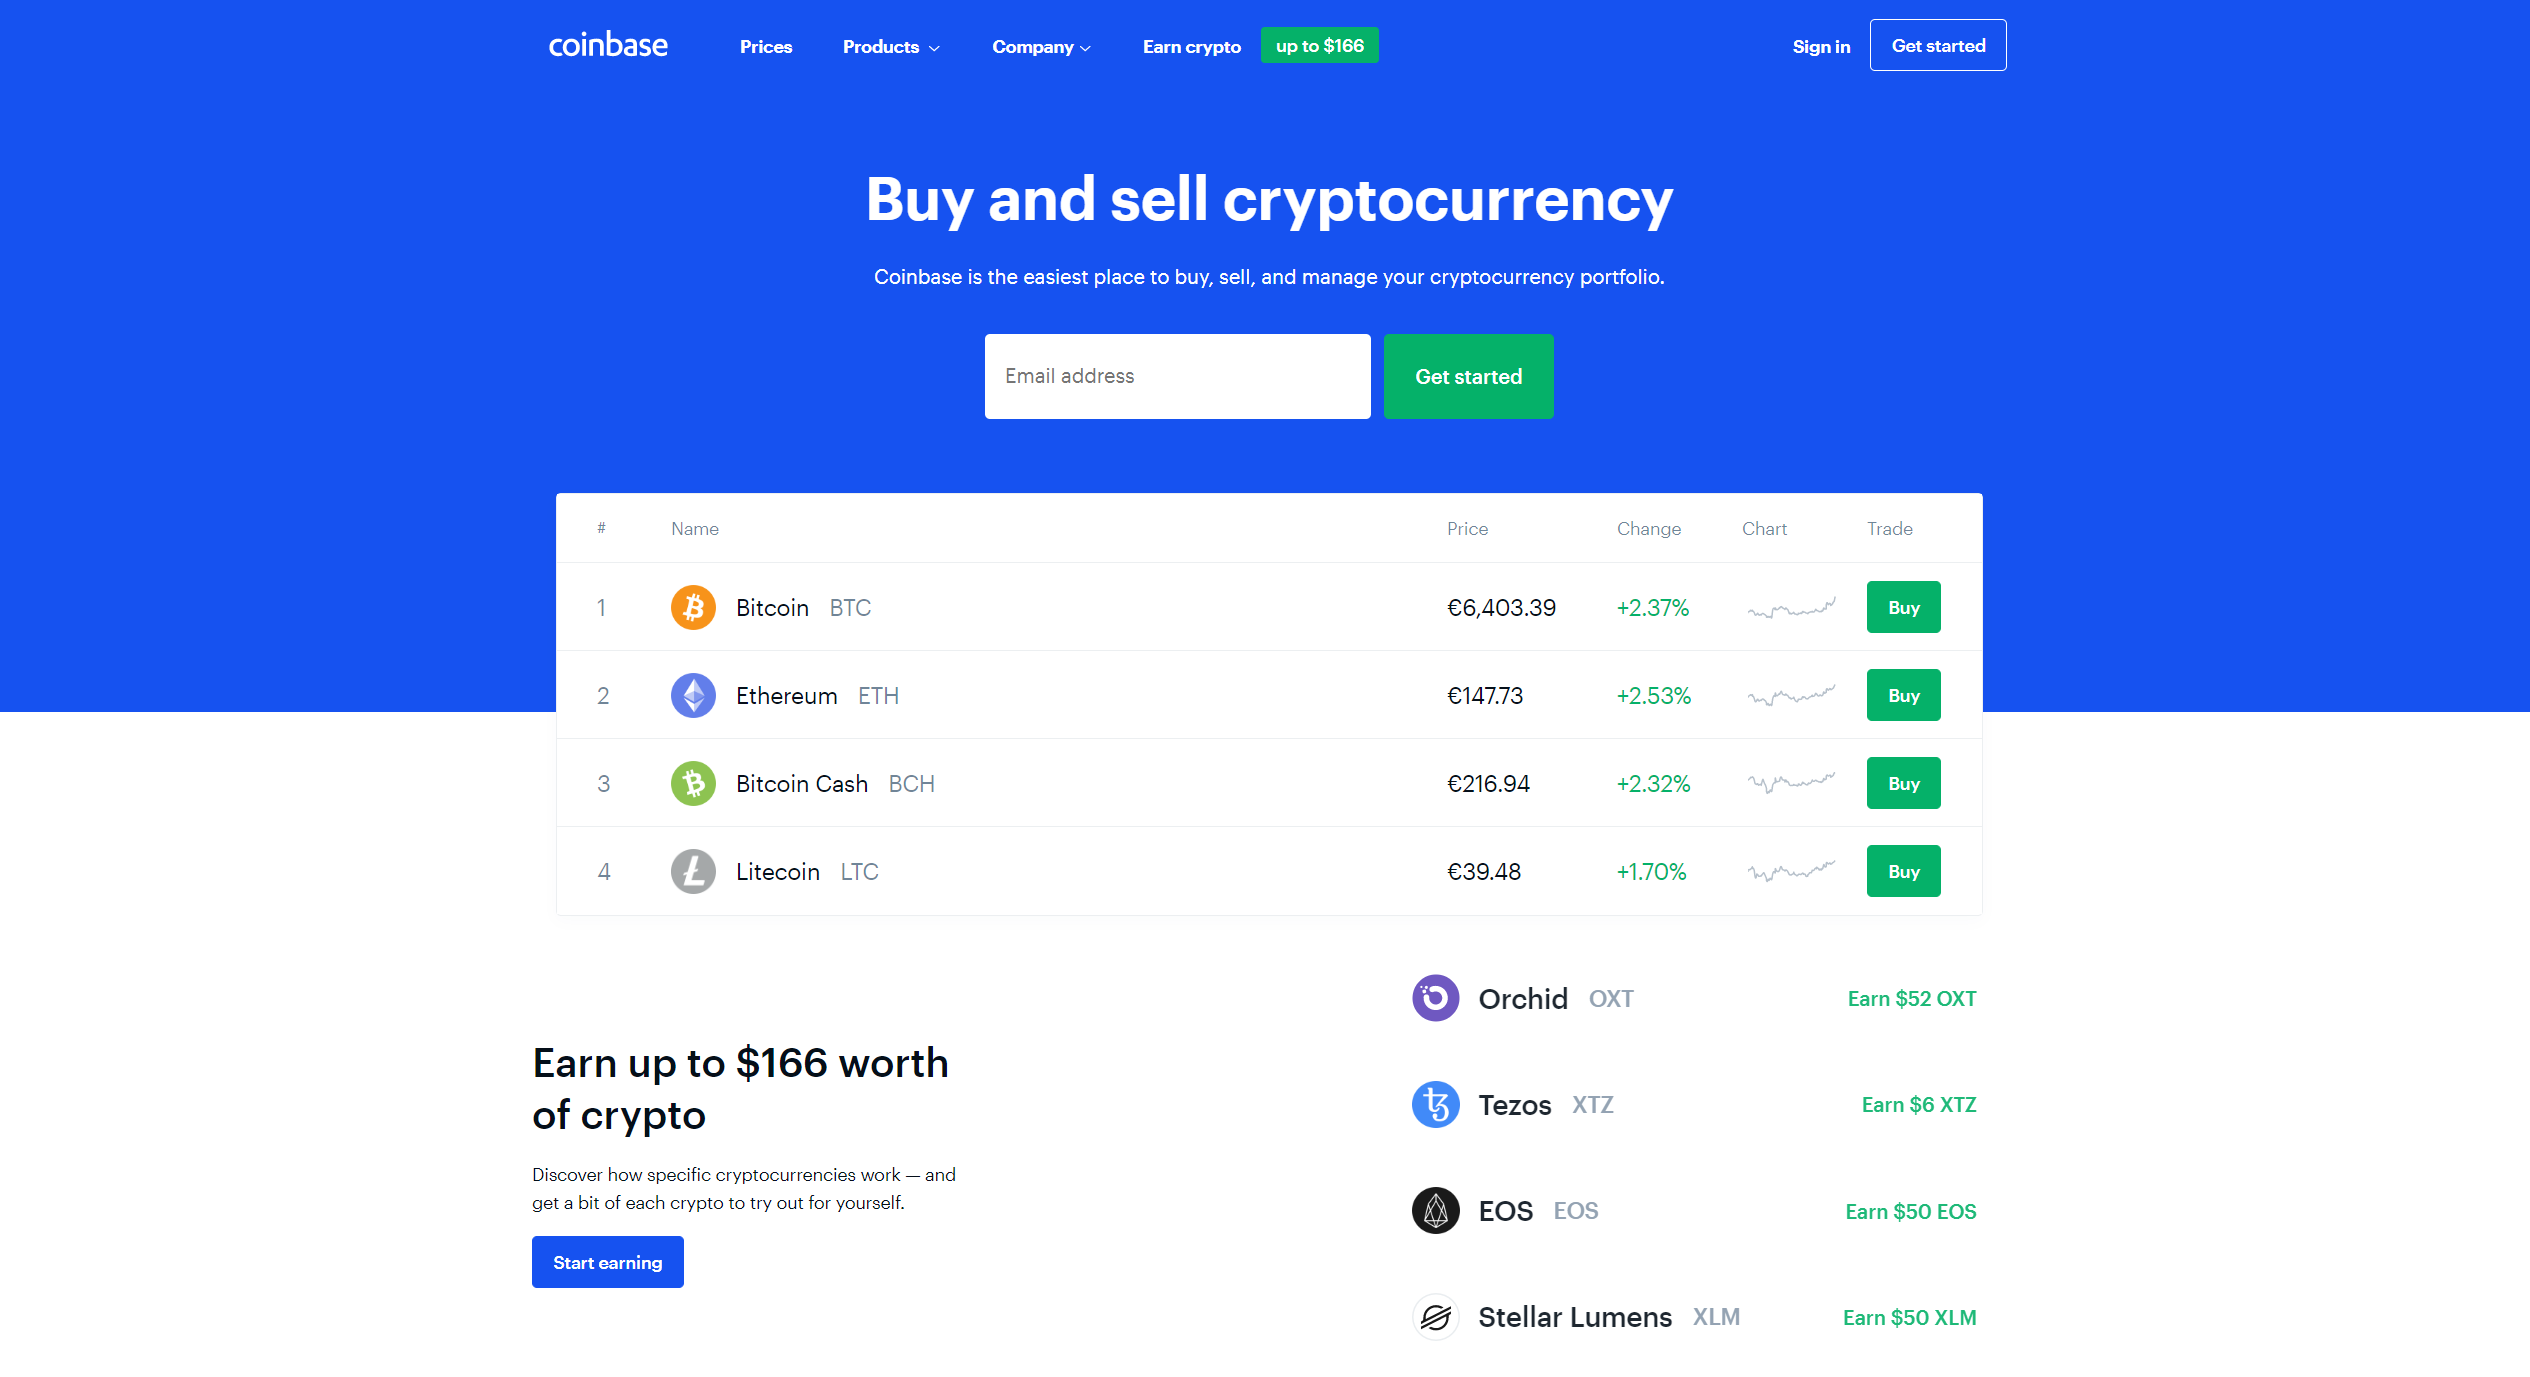
\includegraphics[width=\textwidth]{img/ch-exchanges/coinbase.png}
    \end{borderbox}

\subsection*{Liquid}
\href{https://www.liquid.com?affiliate=nUfQhVL4164547}{Liquid} is a unified, globally-sourced trading platform that bridges the worlds of fiat and crypto. A platform, which offers high liquidity through their \say{World Book}, which connects liquidity pools from exchanges around the world. They also offer a wide range of fiat currency deposits and withdrawals, at very low fees and are fully regulated with a very intuitive user interface and user experience. Also, their native token QASH will provide you with 50\% trading discounts, and you can stake (lend) your tokens to margin traders on the platform to earn interest.

\subsection*{Kraken}
\href{https://www.kraken.com/}{Kraken} was founded in 2011 and is known as one of the largest and oldest Bitcoin exchanges in the world. Kraken is consistently named one of the best places to buy and sell crypto online and has recently updated its website and UI/UX interfaces to appeal to a larger audience. 

\begin{table}[b]

\centering

\caption{Recommended broker and trading exchanges}
\begin{tabular}{llll} 
\toprule

\textbf{Exchange} & \textbf{Type } & \textbf{UX/UI} & \textbf{URL}\\
\midrule

Coinbase & Broker & Beginner & \href{https://www.coinbase.com/join/51954a2b26a1bcc484000015}{https://www.coinbase.com/} \\
KuCoin   &  Trading & Beginner & \href{https://www.kucoin.com/#/?r=aNuPeb}{https://intro.kucoin.com/} \\
Binance  &  Trading & Beginner & \href{https://www.binance.com/?ref=35602166}{https://www.binance.com/en/} \\
Liquid   &  Broker/Trading & Beginner & \href{https://www.liquid.com?affiliate=nUfQhVL4164547}{https://www.liquid.com/} \\
Kraken   &  Broker/Trading & Intermediate & \href{https://www.kraken.com/}{https://www.kraken.com/} \\


\bottomrule
\end{tabular}
\label{tab:exchange selection}
\end{table}

\section{Trading exchanges}
\label{subsec:trading_exchange}

This type of exchange is considered the "traditional" cryptocurrency exchange. It allows you to trade cryptos for other cryptos. For example, if you own Bitcoin and would like to own some Ethereum or other Altcoin, you could sell some of your Bitcoin for something else, using a trading exchange. A trading exchange could be a centralized [CEX] or decentralized exchange [DEX]. We'll list a few in the sections below and indicate if they're decentralized. Remember, these are just some examples - if you want to get the full picture, start with some of the sources listed in \cref{tab:exchangeoverview}.

\subsection*{Binance} 
\href{https://www.binance.com/?ref=35602166}{Binance} is one of the biggest and most popular CEX with huge trade volume and an incredible amount of token listings. It offers a referral program that provides commissions over the trades executed by referrals. It doesn't, however, provide dividends for token holders. Binance is, at the time of writing, a much larger exchange (global 2\textsuperscript{nd}) in terms of volume.
Furthermore, it offers many quality coins, has a very active and involved community and provides many tools for trading. It devotes a considerable sum of its budget to marketing and promotions; hence, it's not surprising that it's one of the largest and fastest-growing exchanges with great potential for the future. 


\subsection*{KuCoin}
\href{https://www.kucoin.com/#/?r=aNuPeb}{KuCoin} is a relatively new player in town which you can compare to Binance. Kucoin has trading incentives in place, essentially sharing 90\% of its trading fees with its users, promoters and investors. It is a competitive new startup based in Hong Kong, and it runs a sleek design, UI/UX interfaces, and an interesting business model. KuCoin pays out its dividend bonuses daily to KuCoin token holders. 

    \bigskip
    \begin{topbox}{TIP}
    KuCoin distributes daily dividend bonuses to KuCoin Shares (KCS) holders. This dividend consists mostly out of the transaction fees of that particular day and is divided proportionally over everyone with KCS stored on the platform (in a custodial wallet).
    \tcblower
    Do you want to know how much you can earn on a daily basis? Visit \href{https://www.stakingrewards.com/asset/kucoin-shares}{stakingrewards}
    \end{topbox}
    
\subsection*{Changelly of Shapeshift}
Cryptocurrency swap platforms such as Changelly and ShapeShift offer an extremely convenient way of trading, with a strong focus on user experience, design, and safety. You choose the crypto to sell and buy, and you can instantly swap tokens and coins. As of recently, there are no more fees on the ShapeShift platform, which is quite amazing.

\paragraph{Changelly} is an instant cryptocurrency exchange platform where you can quickly buy and sell cryptocurrency. You can buy on Changelly using a traditional bank account. Changelly offers competitive crypto-to-crypto rates and supports over 140 cryptocurrencies.

\paragraph{ShapeShift} is the only cryptocurrency trading platform that offers \emph{zero-commission} crypto trading and where the private keys of the trading account are in your control. ShapeShift allows users to purchase crypto with fiat currency and efficiently manage, trade and sell their crypto. Secure your crypto via a beautiful and straightforward web-interface. 

\medskip
\begin{borderbox}
    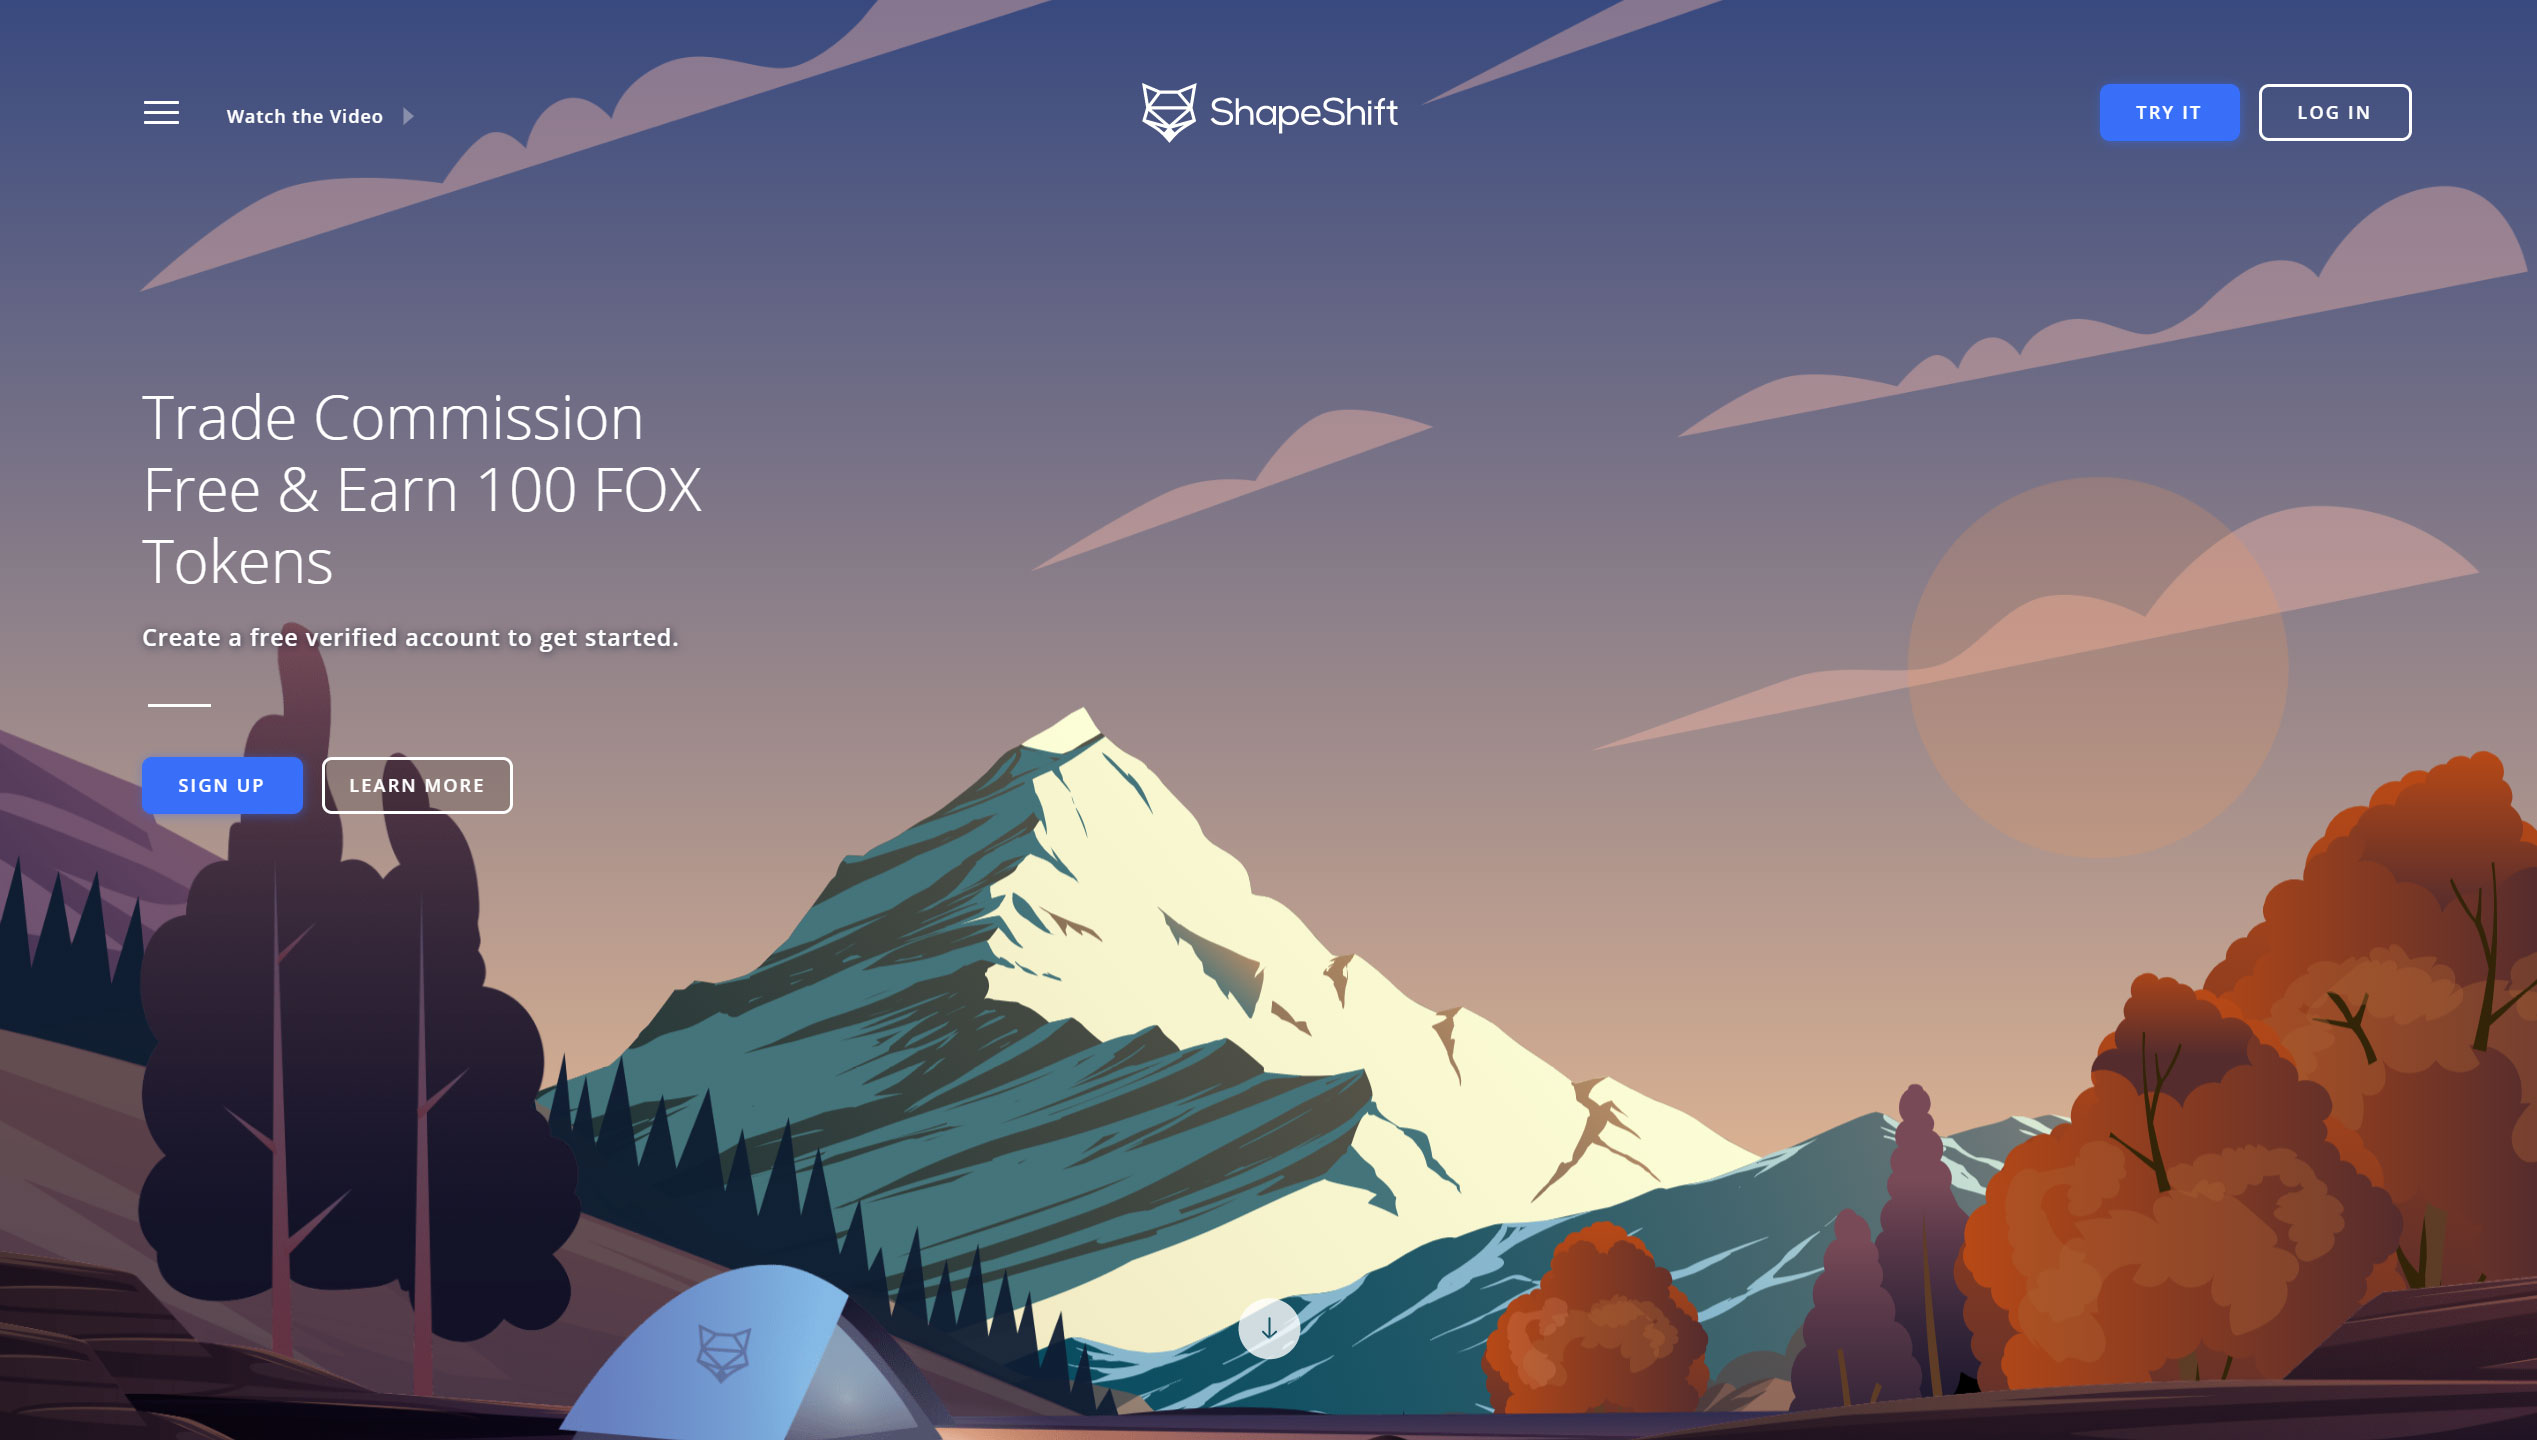
\includegraphics[width=\textwidth]{img/ch-exchanges/ShapeShift.jpg}
\end{borderbox}

\subsection*{Kyber Network (DEX)}
\href{https://www.kyber.network}{Kyber Network} fills a gap in the existing system of cryptocurrency exchanges with its decentralized nature and instant trades. As the number of cryptocurrencies available grows, so will the need for decentralized systems like this, of which Kyber is a pioneer. As more features arrive, including support for arbitrary token pairs, it will become even more helpful for those with cryptocurrency investments.

\medskip
\begin{borderbox}
    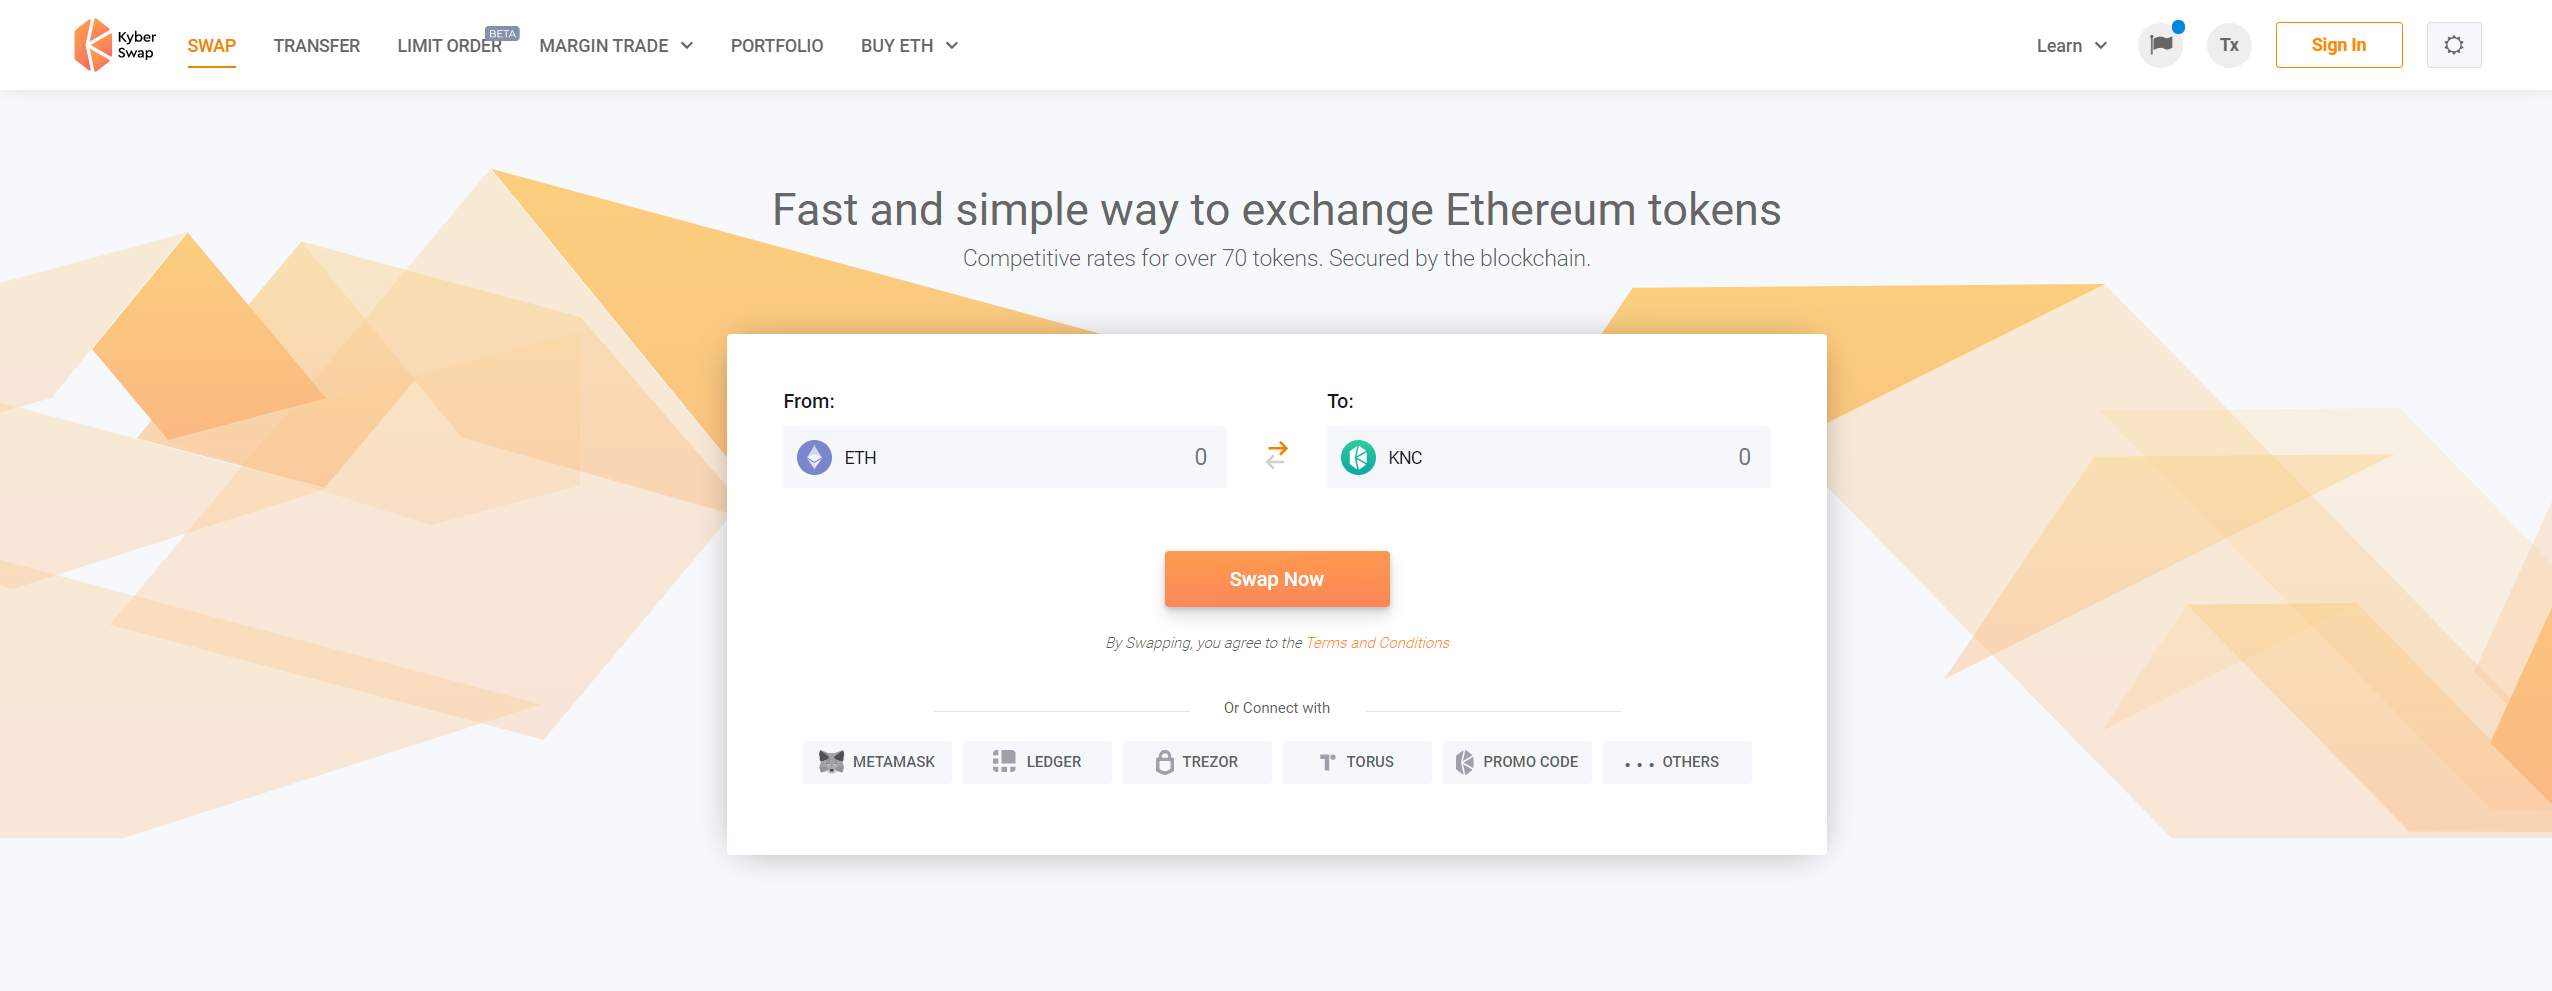
\includegraphics[width=\textwidth]{img/ch-exchanges/kyber_swap.png}
\end{borderbox}

\newpage

\section{Exchange registration \& sign-up}
Signing up for an exchange is relatively straightforward. It is just like registering for any other online service where you need to create an online profile or account. Only now, you are registering for a digital exchange, and you will deposit fiat currency and can start buying and selling cryptocurrency. You must choose the right exchange, so take some time to get familiar with the different types of exchanges, their services, and the pros and cons. Please refer to \cref{sec:exchangetypes} if you're unsure of the kind of exchange you require. In many cases, you'll end up with multiple exchange accounts at some point.

\subsection*{Opening a broker account}
\begin{enumerate}

    \item Open an exchange account and go through all the necessary steps to verify your account.  For more information about the KnowYour Customer (KYC) protocol, refer to section 1.5.
    \item Deposit money from your bank account to your broker exchange account.  Each exchange offers several ways to deposit money.
    \item The exchange notifies you as soon as the money has arrived. Now you can buy Bitcoin, Ethereum or any other cryptocurrency.  

 \end{enumerate}

    \begin{tipbox}{TIP}
              If you intend to purchase cryptocurrency as an investment, you do not need to create an account directly on a trading exchange. Nowadays, many broker exchanges offer quite a lot of trading pairs. If you can buy your cryptocurrency instantly from a broker exchange, you can send it directly to a (hardware) wallet - more about hardware wallets in \cref{ch:wallets}.
    \end{tipbox}
 
\subsection*{Opening a trading account}
 \begin{enumerate}[resume]
    \item Open a trading exchange account at an exchange which offers a variety of other cryptocurrency trading pairs. Usually, these exchanges don't accept any fiat currency deposits. You have to send your crypto o this account from a broker exchange. See \cref{subsec:trading_exchange} for more information about trading exchanges.
    \item After the account is verified, you send the purchased cryptocurrency from the broker account to the trading account. You can then start trading.
    \item You can send a part of the purchased cryptocurrencies directly to the hardware wallet, to keep it safe. Please refer to chapter 2, where we discuss wallet and cryptocurrency trades further. 
\end{enumerate}


\section{Regulation of cryptocurrency exchanges}
Globally, regulators and legislators want to ensure that cryptocurrency exchanges apply both best security practices and measures against criminal activities. These measures discourage illegal activities and also improve the online security of central exchange accounts and the associated cryptocurrency wallets.

\begin{enumerate}
    \item \emph{Know Your Customer} (KYC)
    \item \emph{Anti Money Laundering} (AML)
    \item \emph{Combating the Financing of Terrorism} (CFT)
\end{enumerate} 

Knowing that these regulatory frameworks exist, and what they stand for is essential. Everyone that wishes to participate in regulated cryptocurrency trading and investing will have to prove their identity when registering with an exchange.

\subsection{Know Your Customer (KYC)}
\label{par:KYC}
KYC refers to a set of rules, procedures and processes that exchanges use to identify their customers. When you deposit fiat currency to make purchases and trades, you'll almost always have to verify your identity. This verification can be done in different ways, depending on the nationality and the chosen exchange. It often means that you'll need to upload a photo of yourself with your ID, passport, driver's license or other official documentation.

For low amounts of money, this may not be a requirement - and there is a difference between broker and trading exchanges - but if you plan to deposit and withdraw more substantial amounts of money regularly, you may need to go through several verification stages. Access to a higher level translates into uploading additional personal documents such as bank statements or a rental agreement. This entire process is known as KYC (Know Your Customer).

\subsubsection{ID verification for new users}
Exchanges usually require you to verify your identity. Verifying your identity means you might have to upload a photo of yourself holding your ID, paired with your personal information and bank account details if you wish to deposit currency to start trading. For low amounts of money or low volume trading, this might not be a requirement, and there is a difference between broker and trading exchanges (\cref{sec:exchangetypes}). If you intend to deposit and withdraw more substantial sums of currency regularly, different stages of verification might be required. Higher-level perks translate into uploading personal documents such as bank statements, or driving licenses, addresses and phone numbers (verifying your identity). Completing different stages of KYC could provide you with more perks at the exchange in question concerning maximum deposits, withdrawals, fees and perhaps more. Please refer to the requirements of the centralized exchange which you are interested in. \medskip


\subsection{Anti-Money Laundering (AML)}
AML covers a range of procedures, laws and regulations designed to stop illegal activities such as money laundering. Some of them include tax evasion, market manipulation, misappropriation of public funds, trafficking of illicit goods and other activities of this nature.

AML regulations require financial institutions to carry out ongoing due diligence procedures to detect and prevent malicious activities.

\subsection{Combating the Financing of Terrorism (CFT)}
CFT refers to the series of procedures aimed at investigating, dissecting, discouraging and blocking sources of funding for activities that may be linked to terrorism. This funding is then intended for activities that achieve religious, ideological or political ends through violence, or the threat thereof, against civilians. This set of CFT procedures provides agencies with an alternative and potentially effective way to detect and block terrorist activities in the financial sector.


\newpage

\section{\emph{Best Practices} - crypto exchanges}
\label{sec:importantconsiderations}

The {\fontseries{extrabold}\selectfont Cryptomanual} \say{{\fontseries{medium}\selectfont Best Practices}} provides recommendations and highlights items of importance when considering cryptocurrency exchanges. It is essential to do a little homework before signing up for any exchange. There are a few things you might want to check before making a decision.

\subsection*{Reputation} The best way to find out about an exchange is to search through reviews from individual users and well-known industry websites. You can ask any questions you might have on official social media and community platforms.

\begin{table}[b]

\centering

\caption{Recommended broker and trading exchanges}
\begin{tabular}{llll} 
\toprule

\textbf{Exchange} & \textbf{Type } & \textbf{UX/UI} & \textbf{URL}\\
\midrule

Coinbase & Broker & Beginner & \href{https://www.coinbase.com/join/51954a2b26a1bcc484000015}{coinbase.com} \\
KuCoin   &  Trading & Beginner & \href{https://www.kucoin.com/#/?r=aNuPeb}{intro.kucoin.com} \\
Binance  &  Trading & Beginner & \href{https://www.binance.com/?ref=35602166}{binance.com} \\
Liquid   &  Broker/Trading & Beginner & \href{https://www.liquid.com?affiliate=nUfQhVL4164547}{liquid.com} \\
Kraken   &  Broker/Trading & Intermediate & \href{https://www.kraken.com/}{kraken.com} \\


\bottomrule
\end{tabular}
\label{tab:exchange selection}
\end{table}


\subsection*{Trading pairs}
At the same time, you also look at what affects that trading volume, such as the options in terms of available \emph{trading pairs} such as USD/BTC, USD/ETH, EUR/BTC and EUR/ETH. Bitcoin (BTC) has dominated the cryptocurrency market to date, but there are plenty of other cryptocurrencies - such as Ethereum - with huge trading volumes over 24 hour periods.

\bigskip
\begin{borderbox}
    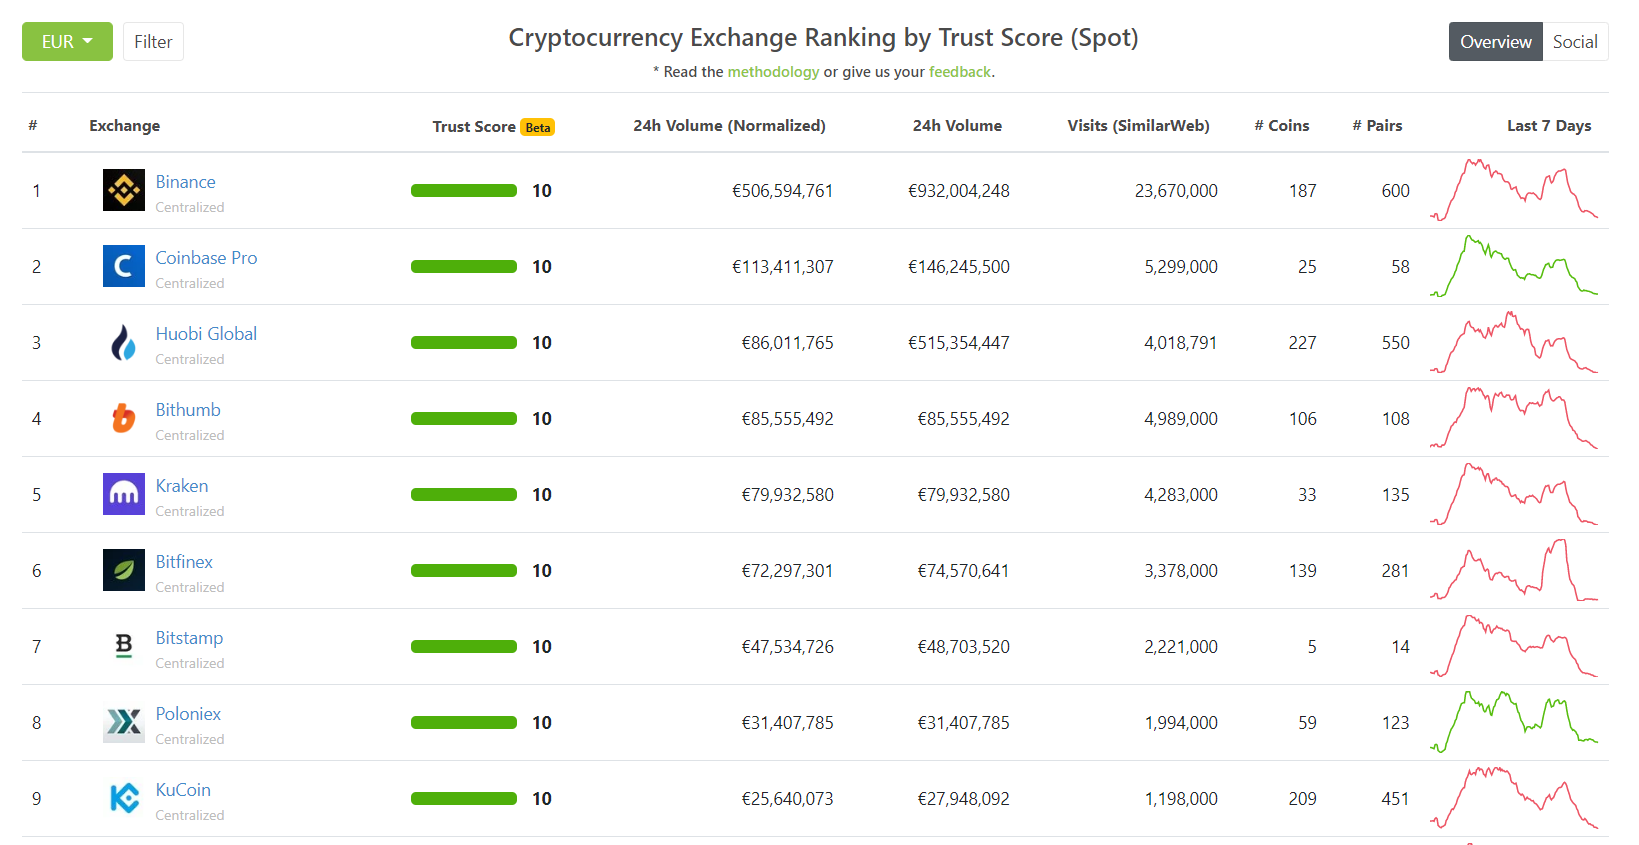
\includegraphics[width=\textwidth]{img/ch-exchanges/exchange-ranking.png}
\end{borderbox}
\medskip

\subsection*{Fees} Most exchanges should have fee-related information on their websites. Before joining, make sure you understand deposit, transaction and withdrawal fees. Fees can differ substantially depending on the exchange you use.

\subsection*{Payment methods} What payment methods are available on the exchange? Credit and debit card? Wire transfer? PayPal? If an exchange has limited payment options, then it may not be convenient for you to use it. Remember that purchasing cryptocurrencies with a credit card will always require identity verification and come with a premium price as there is a higher risk of fraud and higher transaction and processing fees. Purchasing cryptocurrency via wire transfer will take significantly longer as it takes time for banks to process.

\subsection*{Verification requirements} The vast majority of the Bitcoin trading platforms both in the US and the UK require some ID verification to make deposits \& withdrawals. Some exchanges will allow you to remain anonymous. Although verification, which can take up to a few days, might seem like a pain, it protects the exchange against all kinds of scams and money laundering.

\subsection*{Geographical restrictions} Some specific user functions offered by exchanges are only accessible from certain countries. Make sure the exchange you want to join allows full access to all platform tools and services in the country in which you currently live.

\subsection*{Exchange rates} Different exchanges have different rates. You'll be surprised how much you can save if you shop around. It is not uncommon for exchange rates to fluctuate up to 10\% and even higher in some instances.

\newpage

\subsection*{Converting FIAT into cryptocurrency}
 Once registered on an exchange that allows for currency deposits, you can start to engage the market. You now have a host of different options available, depending on the available trading pairs for the currency you deposited. Depending on your country and the currency you're using - you will most likely end up using a broker exchange that operates either internationally and offers multiple currency trading pairs or a local one that also deals in your currency. Trading pairs that you will find almost everywhere would be Bitcoin and Ethereum (USD/BTC, USD/ETH, EUR/BTC, and EUR/ETH). Have a look at the trading pairs available for your currency at your broker exchange. You can deposit money on your exchange account in multiple ways (depending on your provider). You might be able to use bank deposits (SEPA), credit cards or perhaps even services like PayPal.\medskip

As mentioned before, not all types of exchanges accept fiat currency deposits (broker exchanges only); some exchanges only allow you to deposit cryptocurrencies to exchange other alternative coins (trading exchanges). Today, Bitcoin is still one of the most popular cryptocurrencies, and all exchanges offer Bitcoin. Therefore, you can consider it as one of the best gateways for purchasing other coins. In other words, if you want to buy any other cryptocurrencies, you must look at the trading pairs available and do the following:

\begin{enumerate}
    \item Open a (domestic) cryptocurrency broker exchange account (in your country) and verify your account via the "Know Your Customer" (KYC) protocol if required. Please refer to \cref{subsec:broker_exchange} for more information on broker exchanges.
    \item Deposit funds from your bank account to your broker crypto exchange account so you can buy Bitcoin, Ethereum or another coin that has high liquidity and offers multiple trading pairs.
    \item Open a trading exchange account that offers a variety of other cryptocurrencies. Usually, these exchanges do not accept fiat deposits and only allow crypto to crypto trading, withdrawals and deposits. Please refer to \cref{subsec:trading_exchange} for more information on trading exchanges.
    \item After verifying your account, transfer the cryptocurrency that you've bought from your broker exchange to your new trading exchange, and you can start trading. If you don't know how to transfer your freshly purchased coins out of your accounts, please refer to \cref{ch:wallets} where we discuss wallets and transactions.
\end{enumerate}


